\documentclass[12pt]{article}

\usepackage{sbc-template}

\usepackage{graphicx,url}

\usepackage[brazil]{babel}   
\usepackage[utf8]{inputenc}  
   
\sloppy

\title{Avaliação de desempenho de servidores de jogos cooperativos}
\author{Lucas Junqueira Adami (6792496)\inst{1}, Rafael Regis do Prado (6427132)\inst{1}}

\address{
  Instituto de Ciências Matemáticas e de Computação -- Universidade de São Paulo\\
  São Carlos, SP
}

\begin{document} 

\maketitle

\begin{resumo} % 10 linhas
\end{resumo}

\section{Introdução} \label{sec:introcao}

No desenvolvimento de aplicações distribuídas, para a comunicação entre os nós
do sistema, utiliza-se como recurso os \emph{sockets}. No contexto de redes de
computadores, \emph{Sockets} são definidos como interfaces que possibilitam o
fluxo de dados (envio e recebimento de pacotes de dados) entre dois nós por
meio de uma rede, utilizando uma \emph{API} (\emph{Application Programming
Interface} - Interface de Programação de Aplicativos) definida.

Dependendo do contexto em que está sendo aplicado, pode-se utilizar diferentes
modos de operação e protocolos de comunicação. Com relação ao modo de operação,
existem duas formas de se utilizar \emph{sockets}: bloqueante e não bloqueante.
Além disso, pode-se utilizar protocolos que mantém ou não a conexão entre os
nós, como por exemplo os protocolos \emph{TCP} e \emph{UDP}, respectivamente.

Quanto ao modo de operação, ao se realizar uma operação bloqueante, o nó
envolvido interrompe a execução do programa até que o dado em questão seja
enviado ou recebido. Nesse tipo de comunicação, é garantido que todo o pacote
foi devidamente processado a cada operação de E/S (entrada e saída).

Em seu modo não bloqueante, não há o interrompimento da execução ao se utilizar
o \emph{socket}. A aplicação apenas verifica se há dados a serem escritos ou
lidos antes de realizar um comando nesse modo. Como consequência, é possível
que a operação não seja executada por completo. 

Cada modo de operação e protocolo de comunicação possui vantagens, desvantagens
e contextos em que são mais apropriados. Em cenários em que a entrega de todos
os pacotes não seja um requisito, como em aplicações de videoconferência,
protocolos como o \emph{UDP} trazem maior eficiência. Por outro lado,
aplicações bancárias, que necessitam de total integridade de dados, requerem a
utilização de protocolos mais seguros, como o \emph{TCP}.

Em todos os casos, os diferentes modos de operação de \emph{sockets} podem ser
utilizados para se aumentar o desempenho de aplicações em geral. Tal recurso
pode reduzir significativamente o tempo necessário para se finalizar uma
operação de envio e recebimento de dados, possibilitando melhor utilização de
recursos computacionais.

\section{Objetivos} \label{sec:objetivos}

O objetivo deste trabalho é avaliar o desempenho dos diferentes modos de
operação e protocolos de comunicação disponíveis para \emph{sockets} em
aplicações distribuídas. A avaliação será realizada no contexto de jogos
cooperativos por utilizarem \emph{sockets} para que haja sincronia entre todos
os clientes (jogadores) por meio de servidores.

\section{Atividades Desenvolvidas} \label{sec:atividades}

Para a realização do experimento, uma série de procedimentos foram realizados.
Inicialmente foi realizado o planejamento do experimento
(seção~\ref{sub:planejamento}) a ser executado para análise da eficiência de
cada configuração proposta. Em seguida, foi especificado o protocolo de
comunicação entre os clientes e o servidor (seção~\ref{sub:protocolo}) seguido
do desenvolvimento do jogo em si (seção~\ref{sub:desenvolvimento}). Com o jogo
criado, houve a realização dos experimentos e a análise dos resultados
(seção~\ref{sub:realizacao}) para que fosse possível verificar a eficácia de
cada configuração.

\subsection{Planejamento do Experimento} \label{sub:planejamento}

Nesta etapa, foram decididos itens fundamentais para a realização do
experimento. Inicialmente, o tipo de jogo (incluindo a natureza das
comunicações a serem realizadas) foi determinado. O jogo escolhido basea-se no
popular jogo Bomberman, no qual jogadores podem ativar bombas de modo a
estrategicamente atingir outros jogadores com a explosão da mesma.

A partir do jogo escolhido, determinou-se as variáveis do experimento e
cenários que deveriam ser analisados, tais variáveis podem ser analisadas
abaixo. Com isso, foram planejados os experimentos listados na Tabela~\ref{tab:experimentos}.

\begin{itemize}
  \item \textbf{Protocolo de transporte:} Protocolos TCP e UDP.
  \item \textbf{Tipo de comunicação:} Sockets bloqueantes e não bloqueantes.
  \item \textbf{Tamanho dos pacotes transmitidos:} Pacotes com tamanhos na faixa de 0 a 50 e 100 a 150.
  \item \textbf{Número de jogadores simultâneos:} Cenários com 50 e 100 jogadores simultâneos.
\end{itemize}

\begin{table}
  \center
  \footnotesize
  \begin{tabular}{|c|c|c|c|c|}
  \hline
    \#  & \textbf{Protocolo de transporte} & \textbf{Tipo de comunicação} & \textbf{Tamanho do pacote} & \textbf{Jogadores} \\ \hline
    1 & TCP & Não-bloqueante & 0 & 50 \\ \hline
    2 & TCP & Não-bloqueante & 0 & 100 \\ \hline
    3 & TCP & Não-bloqueante & 100 & 50 \\ \hline
    4 & TCP & Não-bloqueante & 100 & 100 \\ \hline
    5 & TCP & Bloqueante & 0 & 50 \\ \hline
    6 & TCP & Bloqueante & 0 & 100 \\ \hline
    7 & TCP & Bloqueante & 100 & 50 \\ \hline
    8 & TCP & Bloqueante & 100 & 100 \\ \hline
    9 & UDP & Não-bloqueante & 0 & 50 \\ \hline
    10 & UDP & Não-bloqueante & 0 & 100 \\ \hline
    11 & UDP & Não-bloqueante & 100 & 50 \\ \hline
    12 & UDP & Não-bloqueante & 100 & 100 \\ \hline
    13 & UDP & Bloqueante & 0 & 50 \\ \hline
    14 & UDP & Bloqueante & 0 & 100 \\ \hline
    15 & UDP & Bloqueante & 100 & 50 \\ \hline
    16 & UDP & Bloqueante & 100 & 100 \\ \hline
  \end{tabular} 
\caption{Experimentos planejados}
\label{tab:experimentos}
\end{table} 

falar do que foi observado

Para a execução dos experimentos, optou-se pela utilização do \textit{cluster}
disponível no Laboratório de Sistemas Distribuídos e Programação Concorrente
(LaSDPC). Nesse sentido, planejou-se utilizar até 11 nós: 1 para o servidor do
jogo e 1 para cada 10 clientes (jogadores). Cada experimento foi planejado para
ser executado 10 vezes, extraindo-se a média das informações obtidas,
totalizando 160 execuções de experimentos.

falar das configuraçoes das maquinas do cluster (servidor é no virtual, clientes são nos fisicos)

\subsection{Especificação do Protocolo} \label{sub:protocolo}

Para possibilitar a simulação de um ambiente de jogos cooperativos com
múltiplos jogadores, foi necessário planejar e especificar um possível
protocolo de aplicação para a interação entre os clientes e o servidor.  Dessa
forma, foi criado um conjunto de 14 ações (Tabela~\ref{tab:protocolo}) que
envolvem o envio de mensagem do cliente para o servidor e do servidor para o
cliente.

\begin{table}
  \center
  \footnotesize
  \begin{tabular}{|c|c|c|c|}
  \hline
    \textbf{ID} & \textbf{Nome} & \textbf{Remetente} & \textbf{Campos (seguido do número de bytes)} \\ \hline
    0 & login & Cliente & Nome Jogador(20)  \\ \hline
    1 & add player & Servidor & Identificador(2), Coordenadas X e Y(4), Nome Jogador(20)\\ \hline
    2 & remove player & Servidor & Identificador(2) \\ \hline
    3 & move me & Cliente & Direção(1) (Ex: Norte=0, Leste=2) \\ \hline
    4 & move player & Servidor & Identificador(2), Coordenadas X e Y(4) \\ \hline
    5 & plant bomb & Cliente & \\ \hline
    6 & add bomb & Servidor &  Identificador(2), Coordenadas X e Y(4)  \\ \hline
    7 & explode bomb & Servidor & Identificador (2) \\ \hline
    8 & fall player & Servidor & Identificador (2) \\ \hline
    9 & acknowledge & Cliente & \\ \hline
   10 & ping & Cliente & \\ \hline
   11 & pong & Servidor & \\ \hline
   12 & info & Cliente & Média(16), Desvio Padrão(16), Pacotes Perdidos(4)  \\ \hline
   13 & shutdown & Servidor &\\ \hline
  \end{tabular} 
\caption{Protocolo do jogo criado}
\label{tab:protocolo}
\end{table} 

Para início de interação, cada cliente deve se apresentar para o cliente
através da ação \textit{login} especificando, inclusive, o nome que pretende
utilizar. Como resposta a uma requisição de login, o servidor envia um pacote
"add player" que contém, entre outros dados, o identificador do cliente
corrente permitindo que este possa distinguir-se dos demais jogadores.

Para cada jogador que realiza uma ação de login, um pacote de "add player" para
os demais clientes para que fiquem cientes da presença de um novo jogador. Além
do identificador, são enviados também o nome do jogador e suas coordenadas X e
Y para que cada cliente possa representá-los graficamente e considerá-los ao
realizar suas ações. Da mesma forma, quando um cliente se desconecta, o
servidor envia um pacote "remove player" para que o jogador com o identificador
seja removido localmente.

Quando um jogador desejar se movimentar, deve ser realizada uma ação de "move
me" com a direção desejada. Como resposta, o servidor envia para todos os
clientes um pacote \textit{move player} indicando a nova posição do jogador em
questão ou ainda um pacote \textit{fall player}, caso o jogador saia da arena
(perdendo o jogo).

O mesmo ocorre com as bombas posicionadas na arena do jogo. Ao decidir armar
uma bomba, o cliente envia um pacote \textit{plant bomb} para o servidor, que
atualiza os demais jogadores por meio do envio de pacotes "add bomb" e "explode
bomb" quando a mesma explodir. Por fim, caso o servidor deva ser desligado, o
mesmo avisa com um pacote \textit{shutdown}.

Como pode-se notar, todo o controle sobre o jogo como a física da movimentação
e as regras do jogo permanecem no servidor, restando aos clientes atualizarem
suas próprias informações com base nas informações passadas pelo servidor. Este
cenário é comumente adotado uma vez que reduz a complexidade, permite maior
sincronia entre os jogadores e evita que jogadores mal-intencionados burlem
regras do jogo. Em contrapartida, há uma grande sobrecarga no servidor, que
deve lidar potencialmente com centenas de jogadores simultâneos sem que haja
grandes atrasos na comunicação e faltas de sincronismo entre jogadores.

As ações de 9 a 11 (Tabela~\ref{tab:protocolo}) são ações de controle. A ação
\textit{acknowledge} foi incluída para uniformizar a utilização dos protocolos
de transporte TCP e UDP. Uma vez que o protocolo UDP não estabelece uma
conexão entre os pares, é essencial para o servidor que o cliente avise
periodicamente que ainda está ativo, com isso, caso não esteja, o servidor pode
descartá-lo de sua tabela de clientes conectados.

As ações de controle \textit{ping}, \textit{pong} e \textit{info} foram
incluídas com a finalidade de se extrair informações úteis a respeito de
pacotes perdidos e atrasos no envio de pacotes para fins estatísticos, algo
especialmente útil para o projeto de redes em questão.

Periodicamente, o cliente envia um pacote \textit{ping} para o servidor, o qual
imediatamente responde com um pacote \textit{pong} permitindo que o cliente
faça medidas do atraso da comunicação. No final, ao receber um pacote
\textit{shutdown} do servidor, o cliente opcionalmente pode enviar a média e
desvio padrão dos atrasos e a quantidade de pacotes não recebidos (útil quando
se utiliza protocolo UDP para transporte).

\subsection{Desenvolvimento de Jogo Cooperativo} \label{sub:desenvolvimento}

explicar prog que simula n clientes

O servidor desenvolvido possui quatro modos de operação. São eles: \emph{TCP} bloqueante, \emph{TCP} não bloqueante, \emph{UDP} bloqueante e \emph{UDP} não bloqueante. Na Figura~\ref{fig:server}, a maneira como cada modo é implementado é mostrada. Para o \emph{TCP} não bloqueante, há uma única \emph{thread} responsável pelo gerenciamento de todos os \emph{sockets}. Nesse modo, há um \emph{socket} principal, \emph{SS}, que recebe novas conexões. A cada conexão estabelecida, um novo \emph{socket} \emph{Si} é criado para manter a conexão com o cliente \emph{i}. No modo \emph{TCP} bloqueante, há uma \emph{thread} responsável pelo recebimento de novas conexões por meio do \emph{socket} \emph{SS} e duas \emph{threads} de leitura e escrita para cada cliente. Ambos os modos que utilizam \emph{TCP} identificam seus clientes por meio do \emph{file descriptor} (\emph{FD}) do \emph{socket} aberto na conexão. Para o \emph{UDP} não bloqueante, o único \emph{socket} utilizado é o \emph{SS}. Há uma única \emph{thread} responsável por processar pacotes recebidos e a serem enviados. Nos modos \emph{UDP}, não há conexão. Portanto, não existe um \emph{FD} para cada cliente. Desta forma, os clientes são identificados pelo par \emph{IP} e porta no servidor. No modo \emph{UDP} bloqueante, há uma \emph{thread} responsável pela leitura de pacotes de todos os clientes por meio do \emph{socket} \emph{SS} e uma \emph{thread} de escrita para cada cliente e que compartilha o \emph{socket} \emph{SS}. 

\begin{figure}[ht]
\centering
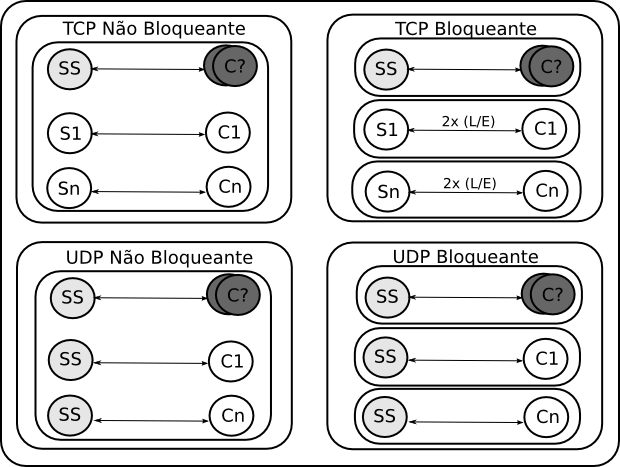
\includegraphics[width=.8\textwidth]{img/server.png}
\caption{Modos de operação do servidor}
\label{fig:server}
\end{figure}

\subsection{Realização de Experimentos e Análise dos Resultados} \label{sub:realizacao}

A partir do jogo desenvolvido, cada um dos 16 experimentos foi executado 10
vezes no \textit{cluster}, como especificado em~\ref{sub:planejamento}. Foram
criados e distribuídos para os nós do cluster uma série de \textit{scripts}
com os parâmetros de interesse devidamente especificados (número de clientes a
serem iniciados na máquina, protocolo de transporte etc).

Com isso, a partir de um determinado nó do \textit{cluster}, o servidor do jogo
foi criado e, por meio de acessos SSH automatizados, os clientes foram criados
em outros nós em seguida, todo o processo conforme o especificado para o
experimento selecionado.

Para cada execução de experimento, foram armazenados dados como a quantidade
total de pacotes trocados entre o servidor e seus clientes, a carga da CPU
durante o experimento, a média e desvio padrão do atraso na comunicação e a
quantidade de pacotes perdidos em disco para análise posterior. Desse total de
dados, foram extraídas as informações de interesse por meio de
\textit{scripts}.

Os resultados obtidos podem ser observados em~\ref{sub:dados} e as conclusões a
respeito dos mesmos podem ser analisadas em~\ref{sub:discussao}.

FALAR DE DIFICULDADES ETC?

\section{Resultados} \label{sec:resultados}
\subsection{Dados Obtidos} \label{sub:dados}

\begin{table}
  \center
  \footnotesize
  \begin{tabular}{|c|c|c|c|c|}
  \hline
    \# & \textbf{Atraso Médio ($ms$)} & \textbf{Variância ($ms$)} & \textbf{CPU usuário/kernel/total (\%)} & \textbf{Bytes enviados/recebidos} \\ \hline
    1 &  &  &  &  \\ \hline
    2 &  &  &  &  \\ \hline
    3 &  &  &  &  \\ \hline
    4 &  &  &  &  \\ \hline
    5 &  &  &  &  \\ \hline
    6 &  &  &  &  \\ \hline
    7 &  &  &  &  \\ \hline
    8 &  &  &  &  \\ \hline
    9 &  &  &  &  \\ \hline
    10 &  &  &  &  \\ \hline
    11 &  &  &  &  \\ \hline
    12 &  &  &  &  \\ \hline
    13 &  &  &  &  \\ \hline
    14 &  &  &  &  \\ \hline
    15 &  &  &  &  \\ \hline
    16 &  &  &  &  \\ \hline
  \end{tabular} 
\caption{Experimentos planejados}
\label{tab:experimentos}
\end{table} 

\subsection{Discussão dos Resultados} \label{sub:discussao}
\section{Conclusões} \label{sec:conclusoes}
% \section{Referências} \label{sec:referencias}

% \begin{figure}[ht]
% \centering
% \includegraphics[width=.5\textwidth]{fig1.jpg}
% \caption{A typical figure}
% \label{fig:exampleFig1}
% \end{figure}

\bibliographystyle{sbc}
\bibliography{bibliography}

\end{document}
